\documentclass[aspectratio=169]{../latex_main/tntbeamer}  % you can pass all options of the beamer class, e.g., 'handout' or 'aspectratio=43'
\usepackage{dsfont}
\usepackage{bm}
\usepackage[english]{babel}
\usepackage[T1]{fontenc}
%\usepackage[utf8]{inputenc}
\usepackage{graphicx}
\graphicspath{ {./figures/} }
\usepackage{algorithm}
\usepackage[ruled,vlined,algo2e,linesnumbered]{algorithm2e}
\usepackage{hyperref}
\usepackage{booktabs}
\usepackage{mathtools}

\usepackage{amsmath,amssymb}

\DeclareMathOperator*{\argmax}{arg\,max}
\DeclareMathOperator*{\argmin}{arg\,min}

\usepackage{amsbsy}
\newcommand{\vect}[1]{\bm{#1}}
%\newcommand{\vect}[1]{\boldsymbol{#1}}

\usepackage{pgfplots}
\pgfplotsset{compat=1.16}
\usepackage{tikz}
\usetikzlibrary{trees} 
\usetikzlibrary{shapes.geometric}
\usetikzlibrary{positioning,shapes,shadows,arrows,calc,mindmap}
\usetikzlibrary{positioning,fadings,through}
\usetikzlibrary{decorations.pathreplacing}
\usetikzlibrary{intersections}
\pgfdeclarelayer{background}
\pgfdeclarelayer{foreground}
\pgfsetlayers{background,main,foreground}
\tikzstyle{activity}=[rectangle, draw=black, rounded corners, text centered, text width=8em]
\tikzstyle{data}=[rectangle, draw=black, text centered, text width=8em]
\tikzstyle{myarrow}=[->, thick, draw=black]

% Define the layers to draw the diagram
\pgfdeclarelayer{background}
\pgfdeclarelayer{foreground}
\pgfsetlayers{background,main,foreground}

% Requires XeLaTeX or LuaLaTeX
%\usepackage{unicode-math}

\usepackage{fontspec}
%\setsansfont{Arial}
\setsansfont{RotisSansSerifStd}[ 
Path=../latex_main/fonts/,
Extension = .otf,
UprightFont = *-Regular,  % or *-Light
BoldFont = *-ExtraBold,  % or *-Bold
ItalicFont = *-Italic
]
\setmonofont{Cascadia Mono}[
Scale=0.8
]

% scale factor adapted; mathrm font added (Benjamin Spitschan @TNT, 2021-06-01)
%\setmathfont[Scale=1.05]{Libertinus Math}
%\setmathrm[Scale=1.05]{Libertinus Math}

% other available math fonts are (not exhaustive)
% Latin Modern Math
% XITS Math
% Libertinus Math
% Asana Math
% Fira Math
% TeX Gyre Pagella Math
% TeX Gyre Bonum Math
% TeX Gyre Schola Math
% TeX Gyre Termes Math

% Literature References
\newcommand{\lit}[2]{\href{#2}{\footnotesize\color{black!60}[#1]}}

%%% Beamer Customization
%----------------------------------------------------------------------
% (Don't) Show sections in frame header. Options: 'sections', 'sections light', empty
\setbeamertemplate{headline}{empty}

% Add header logo for normal frames
\setheaderimage{
	% 
\includegraphics[height=\logoheight]{figures/TNT_darkv4.pdf}
	
\includegraphics[height=\logoheight]{../latex_main/figures/luh_logo_rgb_0_80_155.pdf}
	% 
\includegraphics[height=\logoheight]{figures/logo_tntluh.pdf}
}

% Header logo for title page
\settitleheaderimage{
	% 
\includegraphics[height=\logoheight]{figures/TNT_darkv4.pdf}
	
\includegraphics[height=\logoheight]{../latex_main/figures/luh_logo_rgb_0_80_155.pdf}
	% 
\includegraphics[height=\logoheight]{figures/logo_tntluh.pdf}
}

% Title page: tntdefault 
\setbeamertemplate{title page}[tntdefault]  % or luhstyle
% Add optional title image here
%\addtitlepageimagedefault{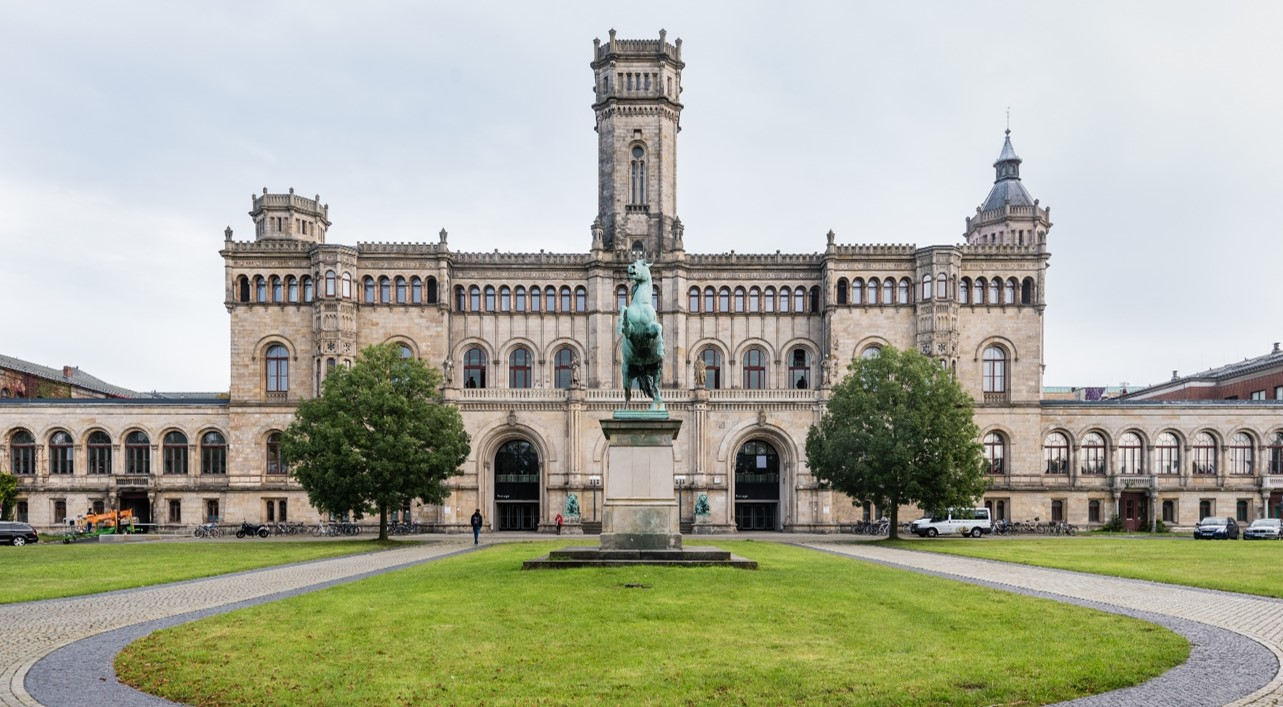
\includegraphics[width=0.65\textwidth]{figures/luh_default_presentation_title_image.jpg}}

% Title page: luhstyle
% \setbeamertemplate{title page}[luhstyle]
% % Add optional title image here
% \addtitlepageimage{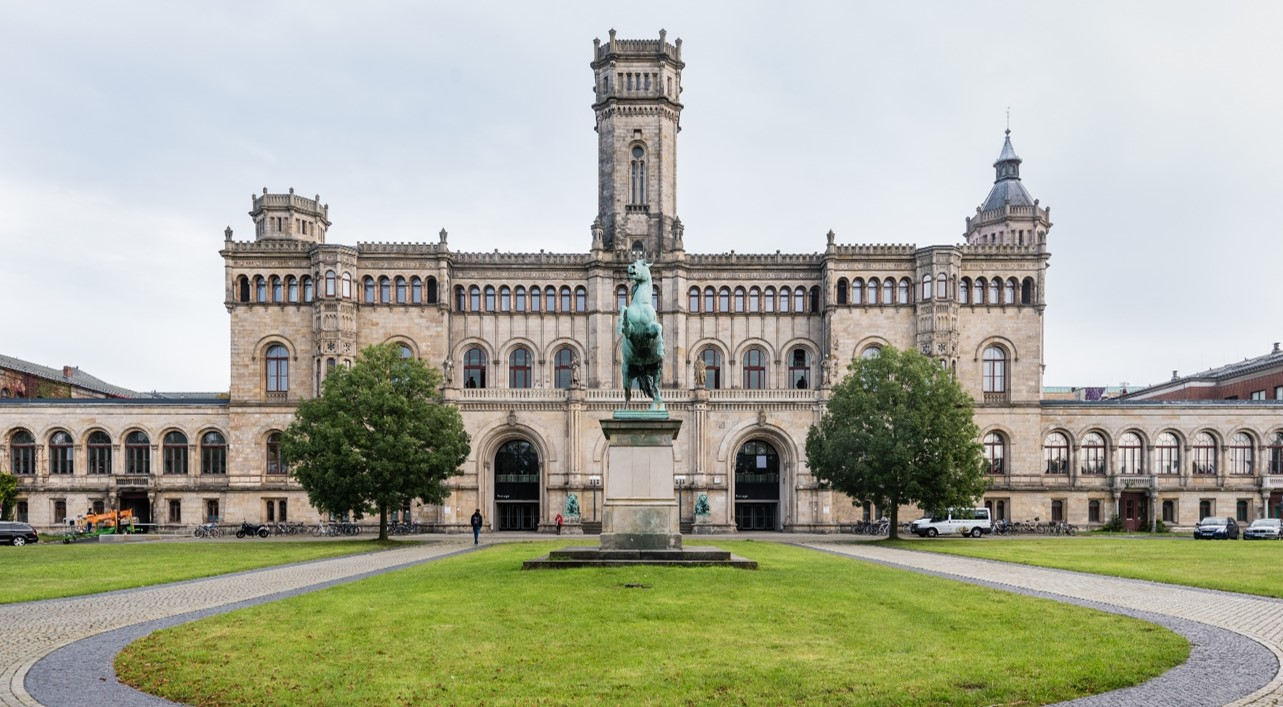
\includegraphics[width=0.75\textwidth]{figures/luh_default_presentation_title_image.jpg}}

\author[Abedjan \& Lindauer]{Ziawasch Abedjan \& Marius Lindauer\\[1em]
	
\includegraphics[height=\logoheight]{../latex_main/figures/luh_logo_rgb_0_80_155.pdf}\qquad
	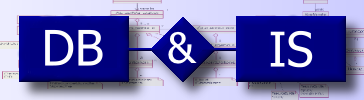
\includegraphics[height=\logoheight]{../latex_main/figures/DBIS_Kurzlogo.png}\qquad

\includegraphics[height=\logoheight]{../latex_main/figures/TNT_darkv4}\qquad

\includegraphics[height=\logoheight]{../latex_main/figures/L3S.jpg}	}
\date{Summer Term 2022; \hspace{0.5em} {
\includegraphics[height=1.5em]{../latex_main/figures/Cc-by-nc-sa_icon.svg.png}}; based on \href{https://ds100.org/fa21/}{[DS100]}
}


%%% Custom Packages
%----------------------------------------------------------------------
% Create dummy content
\usepackage{blindtext}

% Adds a frame with the current page layout. Just call \layout inside of a frame.
\usepackage{layout}


%%% Macros
%\renewcommand{\vec}[1]{\mathbf{#1}}
% \usepackage{bm}
%\let\vecb\bm

\title[Introduction]{DS: Clustering, Part 2}
\subtitle{Graphs}

\graphicspath{ {./figure/} }
%\institute{}


\begin{document}
	
	\maketitle
	\begin{frame}{A New Data Structure}
	    Almost all of the data we’ve worked with so far has been in a rectangular (tabular) format.
	    \begin{itemize}
	        \item Rows are individuals, columns are features, which contain data about the individuals
	        \item If our data wasn’t in rectangular format (rare), we would convert it into a table
	    \end{itemize}
	    \bigskip
	    But not all data fits this structure easily… This is not the only shape data can take!
	    \bigskip
	    Instead of defining an individual by its features, we can define an individual by its relationships with other individuals. We will create a new data structure, called a graph.
	\end{frame}
	
	
	\begin{frame}{Graph}
	    Previously, our data was defined by individuals with input features,   $x_i$    and response $y_i$
	    \begin{itemize}
	        \item Each individual occupied some coordinate in a Euclidean space
	    \end{itemize}
	    \bigskip
	    New data structure: a graph
        Now, our “data points” are vertices, which are connected to each other with edges
        \begin{columns}
            \begin{column}{.5\textwidth}
                    \begin{itemize}
                        \item Each individual vertex is defined by its edges to other vertices
                        \item For our purposes, each edge will have a weight
                        \begin{itemize}
                            \item Stronger weight: the two vertices are more closely connected
                        \end{itemize}
                        \item Possible to give vertices weights as well, but we won’t
                    \end{itemize}
            \end{column}
            
            
            \begin{column}{.5\textwidth}
                    \begin{figure}
                        \centering
                        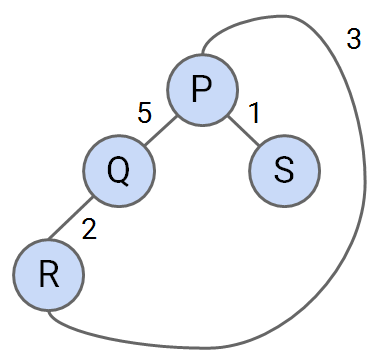
\includegraphics[scale=.4]{Bild4}
                    \end{figure}
            \end{column}
        \end{columns}
	\end{frame}
	
	
	
	\begin{frame}{Displaying a Graph}
	    A graph is NOT defined by the physical coordinates on which it is displayed.
        \begin{columns}
            \begin{column}{.5\textwidth}
                    Tabular Data\\
                    The two datasets below are different.
                    \begin{figure}
                        \centering
                        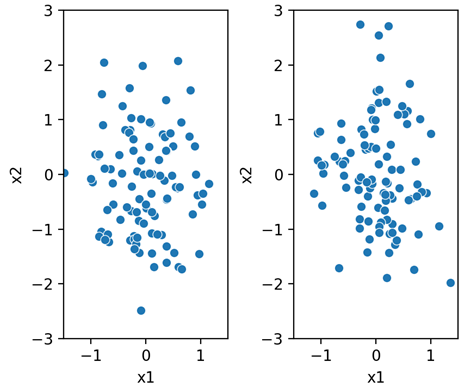
\includegraphics[scale=.45]{Bild5}
                    \end{figure}
            \end{column}
            
            
            \begin{column}{.5\textwidth}
                Graph\\
                The two graphs below are the same, even though they are displayed differently.
                    \begin{figure}
                        \centering
                        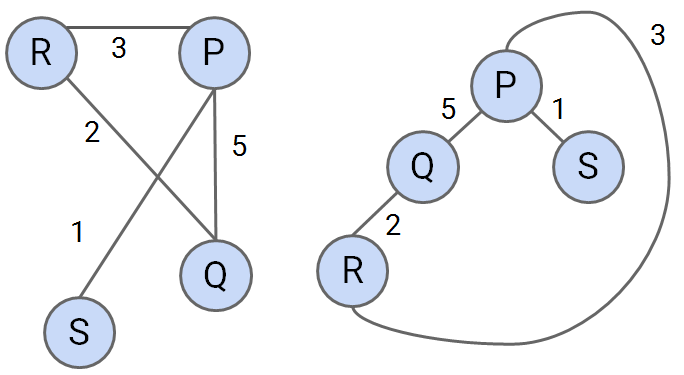
\includegraphics[scale=.4]{Bild6}
                    \end{figure}
            \end{column}
        \end{columns}
	\end{frame}
	
	
	\begin{frame}{Graphical Data}
	    \begin{columns}
            \begin{column}{.5\textwidth}
                    What kind of data might a graph represent?
                    \\\bigskip
                    Example: LinkedIn
                    \begin{itemize}
                        \item Vertices: LinkedIn profiles
                        \item Edges: Whether or not the two profiles are connected
                    \end{itemize}
                    \bigskip
                    Example: UC Berkeley students and the classes they take
                    \begin{itemize}
                        \item Vertices: Individual students
                        \item Edges: How many classes the two students took together
                    \end{itemize}
            \end{column}
            
            
            \begin{column}{.5\textwidth}
                    \begin{figure}
                        \centering
                        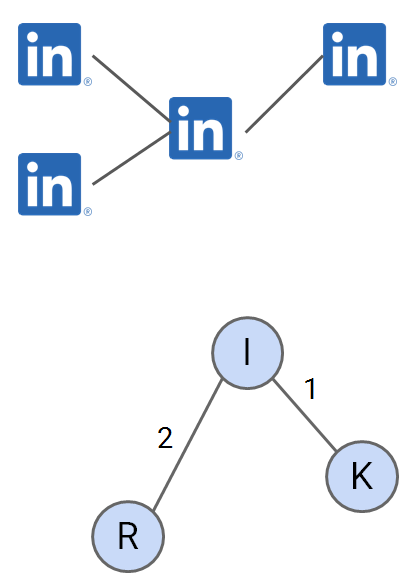
\includegraphics[scale=.35]{Bild7}
                    \end{figure}
            \end{column}
        \end{columns}
	\end{frame}
	
	
	\begin{frame}{.}
	    \begin{figure}
	        \centering
	        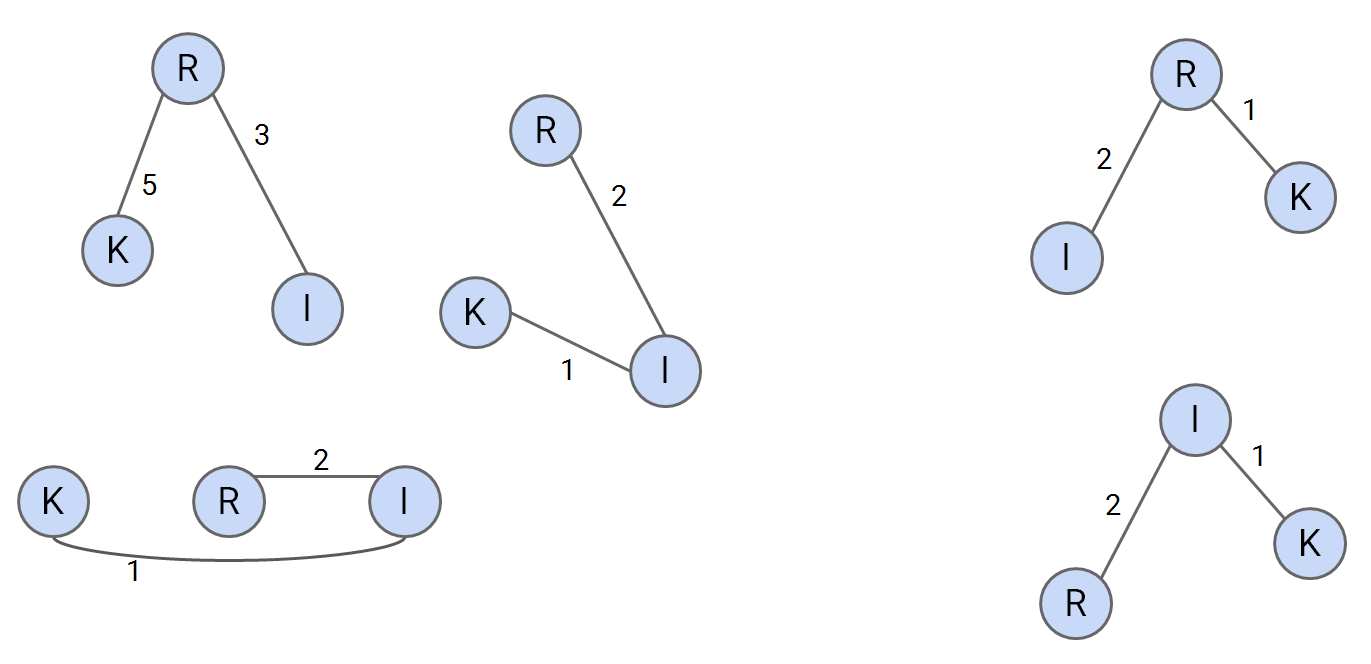
\includegraphics[scale=.35]{Bild8}
	    \end{figure}
	\end{frame}
	
	
	\begin{frame}{Why Graphs?}
	    Q: How might we use graphs to cluster individual data points?\\
	    A: A subset of vertices might be very “dense,” meaning they have lots of edges between them, and/or these edges might have very high weights. These vertices might belong in their own cluster.
	    \begin{figure}
	        \centering
	        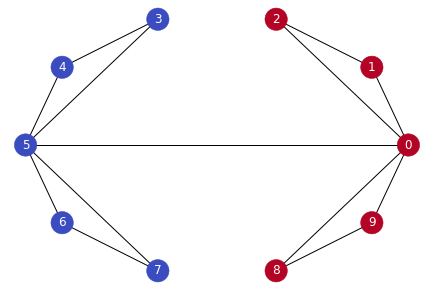
\includegraphics[scale=.65]{Bild9}
	    \end{figure}
	\end{frame}
	
	
	\begin{frame}{Why Graphs?}
	    Graphs lend themselves very nicely to clustering problems.\\
        We can find regions of a graph which are more dense than others
        \begin{itemize}
            \item By “density,” we mean “lots of edges”
        \end{itemize}
       \bigskip
       For example:
       \begin{itemize}
           \item Students who take more classes together may be more likely to have the same major.
           \item Scholars who routinely cite certain other scholars might be researching the same topics.
           \item Movies that cast the same actors might be of similar genres.
       \end{itemize}
       
	\end{frame}
	
	
	
	
	\begin{frame}{Graph Problems}
	    For our purposes, we’ll just use graphs as a tool for clustering.\\
        But graphs have many other applications and can solve many other problems:
        \begin{itemize}
            \item What is the shortest path between two locations?
            \item Does there exist a path that uses each edge exactly once?
            \item Does there exist a path that visits each vertex exactly once?
            \item Which web page should be at the top of a Google search?
            \item How much of each product should each store stock?
        \end{itemize}
        \bigskip
        We will not discuss these problems here. If you are interested, take a look at CS 61B/70/170
	\end{frame}
	
	
	
	\begin{frame}{.}
	     \begin{figure}
	         \centering
	         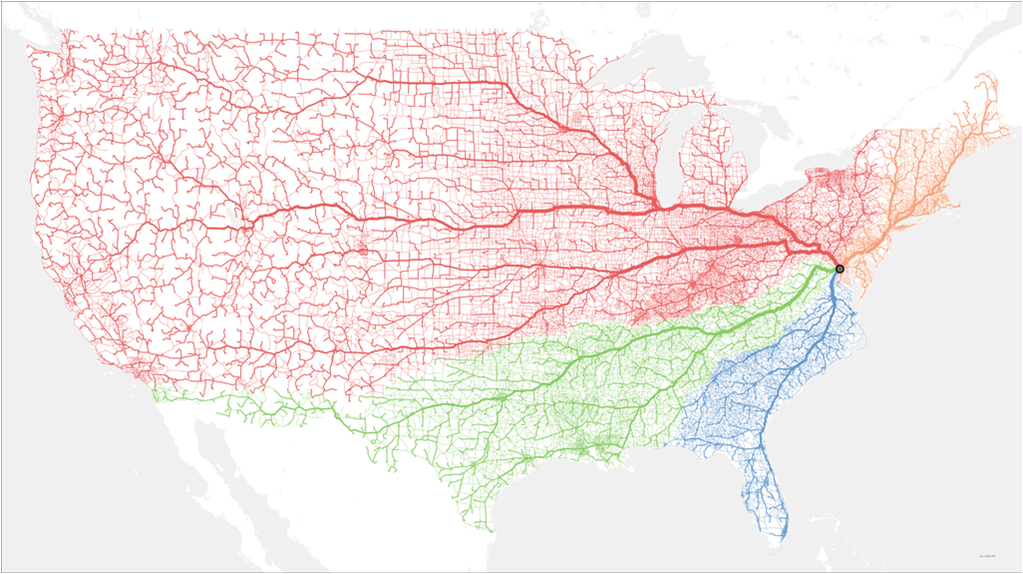
\includegraphics[scale=.485]{Bild10}
	     \end{figure}
	\end{frame}
 \end{document}